\section{Metodologia}\label{sec:metodo}

\subsection{Visão geral}\label{sec:visao}
A Figura~\ref{fig:pipeline} resume a abordagem. Na fase \emph{offline}, a metade de treino (sem rótulos) é
limpa, binarizada por uma codificação em termômetro, resumida em $K$ protótipos, e esses protótipos são gravados
na matriz de pesos $W$. Na fase \emph{online}, cada observação é codificada, a rede a leva a um estado estável e
a diferença entre o estado inicial e o recuperado (ou a energia) vira um escore de anomalia, que um limiar
converte em $\hat y_t$. Rótulos só são usados para escolher o limiar e para avaliar (Seção~\ref{sec:divisao}).

\begin{figure}[htbp]
\centering
\begin{tikzpicture}[node distance=6mm,
  box/.style={draw,rounded corners=2pt,thick,minimum width=25mm,minimum height=9mm,align=center,
              font=\footnotesize,fill=blue!6},
  mem/.style={box,fill=orange!18},
  arr/.style={-{Stealth[length=2mm]},thick},
  dotarr/.style={-{Stealth[length=2mm]},thick,dashed,gray!70!black}]
  \node[box] (pre) {limpeza e\\preparação};
  \node[box,right=of pre] (cod) {codificação\\em termômetro};
  \node[box,right=of cod] (pro) {protótipos\\($K$ padrões)};
  \node[mem,right=of pro] (mem) {memória $W$\\(Hebb/Storkey)};
  \draw[arr] (pre)--(cod);
  \draw[arr] (cod)--(pro);
  \draw[arr] (pro)--(mem);
  \node[anchor=south west,font=\footnotesize\bfseries,text=blue!50!black]
    at ($(pre.north west)+(0,2mm)$) {Fase offline (treino, sem rótulos)};

  \node[box,below=14mm of pre] (obs) {observação\\$x_t$};
  \node[box,right=of obs] (cod2) {codificação\\$s^{0}$};
  \node[box,right=of cod2] (rec) {recuperação\\assíncrona $\sstar$};
  \node[box,right=of rec] (esc) {escore\\$a(x_t)$};
  \node[box,right=of esc,minimum width=17mm] (dec) {$a>\tau$?\\$\hat y_t$};
  \draw[arr] (obs)--(cod2);
  \draw[arr] (cod2)--(rec);
  \draw[arr] (rec)--(esc);
  \draw[arr] (esc)--(dec);
  \node[anchor=north west,font=\footnotesize\bfseries,text=blue!50!black]
    at ($(obs.south west)+(0,-2mm)$) {Fase online (inferência)};

  \draw[dotarr] (cod.south)--(cod2.north);
  \draw[dotarr] (mem.south)--++(0,-5mm)-|(rec.north);
\end{tikzpicture}
\caption{Pipeline do detector. Setas tracejadas: parâmetros aprendidos \emph{offline} (limiares da codificação
e matriz de pesos) e reutilizados \emph{online}.}
\label{fig:pipeline}
\end{figure}

\subsection{Preparação e limpeza}\label{sec:prep}
\begin{enumerate}
  \item \textbf{Verificação por máquina:} dimensões ($n\times38$), valores ausentes, valores fora de $[0,1]$,
        linhas duplicadas e coerência entre o número de linhas do teste e o do arquivo de rótulos. Na máquina
        1-1 não há problemas (Seção~\ref{sec:smd}). Se houver valores ausentes em outras máquinas, serão
        preenchidos com o último valor válido, nunca com estatísticas do teste.
  \item \textbf{Ordem temporal preservada:} nada é embaralhado.
  \item \textbf{Sem normalização adicional:} os valores já estão em $[0,1]$. Os modelos que exigem
        padronização (SVM, MLP, \emph{k}-NN, OC-SVM) usam média e desvio-padrão calculados \emph{apenas} no
        treino; atributos constantes recebem escala~1, de modo que um desvio no teste continue visível.
  \item \textbf{Atributos constantes} no treino são mantidos e tratados por um bit de novidade
        (Seção~\ref{sec:codificacao}).
  \item \textbf{Treino sem remoção de \emph{outliers}:} sem rótulos, não há como identificar com segurança as
        anomalias eventualmente presentes no treino; a mitigação é a seleção de protótipos com descarte de
        grupos muito pequenos (Seção~\ref{sec:prototipos}).
  \item \textbf{Janelas (ablação):} opcionalmente, $x_t$ é ampliado com resumos (média e máximo por atributo) dos
        últimos $w$ minutos, para capturar a dinâmica temporal. O modelo-base usa só a observação instantânea.
\end{enumerate}

\subsection{Codificação binária em termômetro}\label{sec:codificacao}
A rede de Hopfield discreta trabalha com estados em $\{-1,+1\}^N$, enquanto $x_t\in[0,1]^{38}$. Hopfield e
Tank~\cite[p.~145]{hopfieldtank1985} observam que, numa memória prática, é preciso uma transformação que
codifique a informação do mundo real na representação binária da memória. Usamos a codificação em
\emph{termômetro}.

Para cada atributo variável $j$ e um número de níveis $b$, os limiares $\tau_{j,l}$ são os quantis empíricos do
treino de ordem $l/(b+1)$, $l=1,\dots,b$, descartando repetidos e os que não satisfazem
$\min_t x_{t,j}\le\tau<\max_t x_{t,j}$ (assim cada bit varia no treino). O código do atributo é
$s_{j,l}=+1$ se $x_j>\tau_{j,l}$ e $s_{j,l}=-1$ caso contrário. Cada atributo \emph{constante} no treino, com
valor $c_j$, recebe um único \emph{bit de novidade}: $+1$ se $|x_j-c_j|>\varepsilon$ ($\varepsilon=10^{-6}$) e
$-1$ caso contrário. O estado total tem $N=N_{\text{term}}+n_{\text{const}}$ bits.

Uma propriedade útil (derivada no Apêndice~\ref{apx:deriv}): para um mesmo atributo, a distância de Hamming
entre os códigos de dois valores é o número de limiares entre eles, isto é, a diferença de postos
(quantis). A distância de Hamming entre estados completos é, portanto, uma distância \emph{ordinal}, somada
entre atributos, o que a torna insensível à escala de cada atributo.

\begin{table}[htbp]
\centering
\caption{Exploração da codificação em termômetro na máquina 1-1 (metade de treino, 28.479 linhas; cálculo
próprio). ``Padrões distintos'': linhas de treino com códigos diferentes. $\bar s_k$: média do bit $k$ no
treino. A última coluna é a razão entre o número de linhas de treino e a capacidade clássica $0{,}138N$.}
\label{tab:codificacao}
\small
\setlength{\tabcolsep}{4pt}
\begin{tabularx}{\textwidth}{@{}rRRRRRR@{}}
\toprule
$b$ & Bits de termômetro & $N$ (com 8 de novidade) & Padrões distintos & Média dos bits & Média de $|\bar s_k|$ & Treino $/\,(0{,}138N)$\\
\midrule
2  & 59  & 67  & 22.855 & $-0{,}065$ & 0,333 & 3.080\\
4  & 114 & 122 & 27.670 & $-0{,}064$ & 0,405 & 1.692\\
8  & 216 & 224 & 28.459 & $-0{,}040$ & 0,451 & 921\\
16 & 404 & 412 & 28.479 & $-0{,}032$ & 0,480 & 501\\
\bottomrule
\end{tabularx}
\end{table}

A Tabela~\ref{tab:codificacao} traz dois alertas. Primeiro, o número de linhas de treino é de 501 a 3.080
vezes a capacidade clássica: \emph{armazenar todos os pontos é impossível}, e precisamos de $K\ll0{,}138N$
protótipos (ou da rede moderna, com memória grande). Segundo, os bits do termômetro são \emph{viesados por
construção}: o bit do quantil $l/(b+1)$ tem média $1-2l/(b+1)$ no treino, e a média de $|\bar s_k|$ fica entre
0,33 e 0,48. As estimativas de capacidade da Seção~\ref{sec:capacidade} supõem padrões não viesados, logo a
capacidade efetiva deve ser menor que a da Tabela~\ref{tab:capacidade}. Por fim, cada bit de novidade pesa
apenas $1/N$ em $S_1$ (Seção~\ref{sec:escores}), um sinal fraco; combinar o detector com uma regra explícita
é uma extensão possível (Seção~\ref{sec:conclusoes}).

\subsection{Memória de protótipos}\label{sec:prototipos}
Os $K$ padrões armazenados são escolhidos entre os códigos da metade de treino por \emph{k-medoids} no espaço
de Hamming (ou \emph{k-modes}), ajustado sobre uma subamostra de até 5.000 pontos para limitar o custo. Usar
medoides garante que cada protótipo seja um padrão realmente observado. Grupos com menos de uma pequena fração
dos pontos (por exemplo, 1\,\%) podem ser descartados, para diminuir o risco de gravar anomalias que estejam
no treino. Variamos $K\in\{2,5,10,20,30\}$; esse intervalo inclui valores acima da capacidade teórica (por
exemplo, $K=30$ com $N=67$, $K/N\approx0{,}45$) de propósito, para observar a degradação prevista (H1,
Seção~\ref{sec:experimentos}). Os protótipos são gravados com a regra de Hebb~\eqref{eq:hebb} ou de
Storkey~\eqref{eq:storkey}, com $\theta=0$ (Algoritmo~\ref{alg:armazenar}).

\subsection{Recuperação e escores de anomalia}\label{sec:escores}
Dada uma observação $x_t$, o detector (i) calcula $s^{0}=\mathrm{cod}(x_t)$; (ii) executa a recuperação
assíncrona (Algoritmo~\ref{alg:recuperar}): varreduras em ordem aleatória até que uma varredura completa não
altere nenhum bit, com no máximo $T_{\max}=100$ varreduras --- a Proposição~\ref{prop:conv} garante a parada ---
e obtém $\sstar$; (iii) calcula os escores da Tabela~\ref{tab:escores}.

\begin{table}[htbp]
\centering
\caption{Escores de anomalia da rede clássica (quanto maior, mais anômalo). $\xi^\mu$: protótipos
armazenados; $E$: energia~\eqref{eq:energia}. Propostas de projeto.}
\label{tab:escores}
\small
\begin{tabularx}{\textwidth}{@{}lcL@{}}
\toprule
Escore & Definição & Leitura\\
\midrule
$S_1$ & $\hamm(s^0,\sstar)/N$ & fração dos bits alterada pela dinâmica\\
$S_2$ & $\min_\mu\hamm(s^0,\xi^\mu)/N$ & distância ao protótipo mais próximo \emph{sem} dinâmica (referência do vizinho mais próximo no espaço do código)\\
$S_3$ & $E(s^0)$ & energia do estado inicial\\
$S_4$ & $E(s^0)-E(\sstar)$ & energia liberada pela recuperação\\
$S_5$ & $\min_\mu\hamm(\sstar,\xi^\mu)/N$ & distância do estado final ao protótipo mais próximo (alta $\Rightarrow$ estado espúrio ou invertido)\\
$S_6$ & nº de varreduras com ao menos uma troca & tempo de convergência\\
\bottomrule
\end{tabularx}
\end{table}

A comparação entre $S_1$ e $S_2$ mede se a dinâmica recorrente acrescenta algo à simples busca do protótipo
mais próximo (ablação). Usamos a distância \emph{com sinal}, e não o módulo da sobreposição, de modo que o padrão
invertido $-\xi^\mu$ --- que é ponto fixo com a mesma energia de $\xi^\mu$ quando $\theta=0$ (Seção~\ref{sec:capacidade})
--- conte como distante: para uma consulta igual a $-\xi^\mu$, $S_1=0$ e $S_3$ é baixo, mas $S_2=S_5=1$
(Apêndice~\ref{apx:exemplo}).

\paragraph{Variante moderna.} A memória é a matriz $X$ formada pelas linhas de treino (ou por uma subamostra
ou centroides de $k$-means), no espaço contínuo --- atributos em $[0,1]$ ou padronizados, sem normalizar cada
vetor, porque a magnitude carrega informação. Com $\beta\in\{1,10,100,1000\}$ (ou seja, $\sigma=\beta^{-1/2}$),
os escores são $E(\xi^0)$ (Eq.~\ref{eq:energia-moderna}), o resíduo de recuperação
$\|\xi^0-X\softmax(\beta X^{\top}\xi^0)\|$ e a entropia do vetor $\softmax(\beta X^{\top}\xi^0)$
(Algoritmo~\ref{alg:moderna}). O custo por consulta é $O(NK)$ com $N=38$ e $K$ até o número de linhas de treino.
Pela Seção~\ref{sec:moderna}, esperamos que esses escores se comportem como escores de densidade por kernel.

\subsection{Linhas de base}\label{sec:baselines}
O enunciado exige ao menos dois modelos de classificação da lista (\emph{Decision Trees}, \emph{Random Forest},
\emph{Naive Bayes}, SVM, MLP, XGBoost e KNN)~\cite{enunciado}. Como a rede de Hopfield não consta da lista
(Seção~\ref{sec:intro}), tratamo-la como \emph{modelo do tema} e usamos as linhas de base abaixo, implementadas
com o \texttt{scikit-learn}~\cite{pedregosa2011}.
\begin{itemize}
  \item \textbf{Supervisionadas (Etapa~I):} \emph{Random Forest} (com \texttt{class\_weight='balanced'}) e SVM com
        núcleo RBF, treinadas em $L_{\mathrm{tr}}$ (Seção~\ref{sec:divisao}) sobre os 38 atributos originais. São uma
        \emph{referência superior}: usam rótulos, ao contrário do detector \emph{one-class}, e portanto a
        comparação com o Hopfield não é de igual para igual.
  \item \textbf{\emph{One-class} (comparação justa):} \emph{One-Class SVM} e distância ao $k$-ésimo vizinho mais
        próximo (\emph{k}-NN), ajustados apenas na metade de treino sem rótulos, como a rede de Hopfield.
  \item \textbf{Opcional:} MLP (classificador ou autoencoder).
\end{itemize}

\subsection{Divisão dos dados e protocolos de avaliação}\label{sec:divisao}
A metade de treino do SMD não tem rótulos; rótulos --- para treinar modelos supervisionados, escolher
limiares e avaliar --- só existem na metade de teste. Dividimos essa metade \emph{cronologicamente} em três
blocos, nunca por sorteio: pontos vizinhos de uma série temporal são fortemente correlacionados e um sorteio
vazaria informação do teste para o treino. Seja $n$ o número de linhas da metade rotulada,
$c_1=\mathrm{round}(0{,}4\,n)$ e $c_2=\mathrm{round}(0{,}6\,n)$:
\begin{equation}\label{eq:blocos}
L_{\mathrm{tr}}=[0,\,c_1-60),\qquad L_{\mathrm{val}}=[c_1+60,\,c_2-60),\qquad L_{\mathrm{te}}=[c_2+60,\,n),
\end{equation}
com um \emph{embargo} de 60 amostras (1 hora) de cada lado de cada corte, para que nenhuma informação vaze
entre blocos vizinhos. Cada corte é deslocado, se necessário, para a zona mais próxima sem anomalias em
$\pm60$ amostras, de modo que nenhum segmento anômalo atravesse uma fronteira nem caia no embargo. Dos 56
cortes (28 máquinas $\times$ 2), apenas 5 foram deslocados: $c_1$ nas máquinas 2-4 (9.413 em vez de 9.476) e
3-7 (11.431 em vez de 11.482), e $c_2$ nas máquinas 1-1 (16.903 em vez de 17.087), 2-9 (17.346 em vez de 17.233)
e 3-8 (17.336 em vez de 17.222). A metade de treino (sem rótulos) também é dividida em ordem cronológica:
$S_{\mathrm{aj}}$ (primeiros 80\,\%), onde se ajustam os modelos \emph{one-class}, e $S_{\mathrm{cal}}$ (últimos
20\,\%), usada para calibrar o limiar sem rótulos.

\begin{figure}[htbp]
\centering
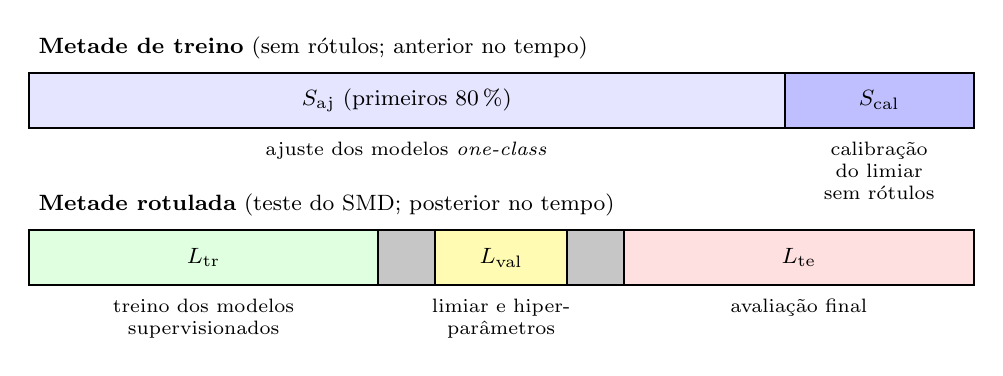
\begin{tikzpicture}[x=12cm,y=1cm,font=\footnotesize]
  \node[anchor=south west] at (0,3.55) {\textbf{Metade de treino} (sem rótulos; anterior no tempo)};
  \draw[thick,fill=blue!10] (0,2.8) rectangle (0.8,3.5);
  \draw[thick,fill=blue!25] (0.8,2.8) rectangle (1,3.5);
  \node at (0.4,3.15) {$S_{\mathrm{aj}}$ (primeiros 80\,\%)};
  \node at (0.9,3.15) {$S_{\mathrm{cal}}$};
  \node[anchor=north,align=center,text width=4cm,font=\scriptsize] at (0.4,2.75)
    {ajuste dos modelos \emph{one-class}};
  \node[anchor=north,align=center,text width=2.2cm,font=\scriptsize] at (0.9,2.75)
    {calibração do limiar sem rótulos};

  \node[anchor=south west] at (0,1.55) {\textbf{Metade rotulada} (teste do SMD; posterior no tempo)};
  \draw[thick,fill=green!12] (0,0.8) rectangle (0.37,1.5);
  \draw[thick,fill=gray!45] (0.37,0.8) rectangle (0.43,1.5);
  \draw[thick,fill=yellow!30] (0.43,0.8) rectangle (0.57,1.5);
  \draw[thick,fill=gray!45] (0.57,0.8) rectangle (0.63,1.5);
  \draw[thick,fill=red!12] (0.63,0.8) rectangle (1,1.5);
  \node at (0.185,1.15) {$L_{\mathrm{tr}}$};
  \node at (0.5,1.15) {$L_{\mathrm{val}}$};
  \node at (0.815,1.15) {$L_{\mathrm{te}}$};
  \node[anchor=north,align=center,text width=3cm,font=\scriptsize] at (0.185,0.75) {treino dos modelos supervisionados};
  \node[anchor=north,align=center,text width=2.2cm,font=\scriptsize] at (0.5,0.75) {limiar e hiperparâmetros};
  \node[anchor=north,align=center,text width=3cm,font=\scriptsize] at (0.815,0.75) {avaliação final};
\end{tikzpicture}
\caption{Divisão cronológica de uma máquina (esquema fora de escala). As faixas cinza são os embargos de
60 amostras, centrados nos cortes $c_1$ e $c_2$.}
\label{fig:divisao}
\end{figure}

\paragraph{Elegibilidade das máquinas.} Nem toda máquina tem anomalias em todos os blocos
(Tabela~\ref{tab:elegib}; números por máquina no Apêndice~\ref{apx:maquinas}). Para treinar um classificador
supervisionado é preciso ter as duas classes em $L_{\mathrm{tr}}$; para escolher o limiar, anomalias em
$L_{\mathrm{val}}$. Por isso o Protocolo~S, descrito abaixo, usa 18 máquinas (e 23 para os modelos
\emph{one-class}), e as 5 restantes entram apenas no Protocolo~U. Alguns $L_{\mathrm{val}}$ têm pouquíssimas
anomalias (máquina 3-5: 3; 2-2: 11; 3-3: 15; 1-8: 16; 3-4: 20; 1-6: 27), de modo que o limiar não é ajustado
por máquina, e sim globalmente, sobre o $L_{\mathrm{val}}$ agregado.

\begin{table}[htbp]
\centering
\caption{Elegibilidade das máquinas, conforme a existência de anomalias em cada bloco (cálculo próprio).}
\label{tab:elegib}
\small
\begin{tabularx}{\textwidth}{@{}lcLL@{}}
\toprule
Classe & Anomalias em $L_{\mathrm{tr}}$ / $L_{\mathrm{val}}$ / $L_{\mathrm{te}}$ & Máquinas & Uso\\
\midrule
S (18) & $>0$ / $>0$ / $>0$ & 1-3, 1-4, 1-6, 1-7, 1-8, 2-1, 2-3, 2-4, 2-5, 2-6, 2-7, 3-2, 3-3, 3-4, 3-5, 3-6, 3-7, 3-10 & Protocolo~S (supervisionados e \emph{one-class})\\
O (5) & $0$ / $>0$ / $>0$ & 1-1, 1-5, 2-2, 2-9, 3-8 & Protocolo~S, só \emph{one-class}\\
-- (5) & $L_{\mathrm{val}}=0$ & 1-2, 2-8, 3-1, 3-9, 3-11 & só Protocolo~U\\
\bottomrule
\end{tabularx}
\end{table}

\begin{table}[htbp]
\centering
\caption{Blocos cronológicos agregados (soma das máquinas de cada conjunto; cálculo próprio).}
\label{tab:blocos}
\small
\begin{tabular}{llrrr}
\toprule
Conjunto & Bloco & Linhas & Anômalas & Prevalência\\
\midrule
\multirow{3}{*}{18 máquinas (S)} & $L_{\mathrm{tr}}$  & 175.448 & 6.664  & 3,80\,\%\\
                                 & $L_{\mathrm{val}}$ & 86.273  & 1.970  & 2,28\,\%\\
                                 & $L_{\mathrm{te}}$  & 175.562 & 10.545 & 6,01\,\%\\
\midrule
\multirow{3}{*}{23 máquinas (S+O)} & $L_{\mathrm{tr}}$  & 228.473 & 6.664  & 2,92\,\%\\
                                   & $L_{\mathrm{val}}$ & 112.377 & 4.500  & 4,00\,\%\\
                                   & $L_{\mathrm{te}}$  & 228.544 & 16.768 & 7,34\,\%\\
\bottomrule
\end{tabular}
\end{table}

A prevalência muda de bloco para bloco (de 2,28\,\% a 6,01\,\% nas 18 máquinas), de modo que um limiar ótimo em
$L_{\mathrm{val}}$ não é necessariamente ótimo em $L_{\mathrm{te}}$; esse é um dos motivos para reportar também
métricas independentes de limiar (AUC-ROC e PR-AUC). Para análises detalhadas e para a Etapa~II escolhemos uma
máquina representativa por grupo, todas com anomalias em todos os blocos: \textbf{1-3}, \textbf{2-5} e \textbf{3-6}
(anomalias em $L_{\mathrm{tr}}$/$L_{\mathrm{val}}$/$L_{\mathrm{te}}$: 86/281/450, 314/39/627 e 174/437/583;
prevalências de 3,45\,\%, 4,14\,\% e 4,16\,\%, próximas dos 4,16\,\% do conjunto).

\paragraph{Limiar de decisão.} Escores de máquinas diferentes não são diretamente comparáveis. Para os modelos
\emph{one-class}, o limiar de cada máquina é o quantil $(1-\alpha)$ dos escores em $S_{\mathrm{cal}}$ ---
isto é, $\alpha$ é a taxa de alarmes tolerada sobre o comportamento normal --- e $\alpha$ é um parâmetro
\emph{global}. Para os modelos supervisionados, o parâmetro global é o limiar sobre a probabilidade prevista.

\begin{table}[htbp]
\centering
\caption{Protocolos de avaliação (propostas de projeto).}
\label{tab:protocolos}
\small
\begin{tabularx}{\textwidth}{@{}lLL@{}}
\toprule
 & Protocolo~S (principal) & Protocolo~U (secundário, sem rótulos)\\
\midrule
Máquinas & 18 (classe S); modelos \emph{one-class} também nas 5 da classe O & 28\\
Ajuste & \emph{one-class}: $S_{\mathrm{aj}}$; supervisionados: $L_{\mathrm{tr}}$ & \emph{one-class}: $S_{\mathrm{aj}}$\\
Limiar e hiperparâmetros & globais, escolhidos por $F_1$ em $L_{\mathrm{val}}$ agregado ($\alpha$ ou limiar de probabilidade) & $\alpha\in\{0{,}5;\,1;\,2;\,5\}\,\%$ fixado \emph{a priori}; limiar por máquina em $S_{\mathrm{cal}}$\\
Avaliação & $L_{\mathrm{te}}$ & toda a metade rotulada\\
Relato & todas as métricas da Seção~\ref{sec:metricas} & AUC-ROC, PR-AUC e métricas no limiar sem rótulos; $F_1$ ótimo (``oráculo'') só como teto otimista\\
\bottomrule
\end{tabularx}
\end{table}

\paragraph{Agregação e significância.} Reportamos a média entre máquinas (\emph{macro}) e as contagens
agregadas (\emph{micro}); a AUC-ROC e a PR-AUC são calculadas por máquina e promediadas. Comparações entre
modelos usam o teste de Wilcoxon dos postos sinalizados, pareado por máquina, e as partes estocásticas (ordem de
atualização, inicialização do \emph{k-medoids}, \emph{Random Forest}, MLP) são repetidas com 3 sementes.

\subsection{Balanceamento de classes}\label{sec:balanceamento}
Com 4,16\,\% de pontos anômalos, o desbalanceamento é forte, mas seu tratamento depende do modelo:
\begin{itemize}
  \item o detector \emph{one-class} (Hopfield, OC-SVM, \emph{k}-NN) não usa rótulos no ajuste, logo não há o que
        balancear;
  \item nos modelos supervisionados usamos pesos de classe (\texttt{class\_weight='balanced'}) ou
        subamostragem da classe majoritária, \emph{apenas em $L_{\mathrm{tr}}$};
  \item não usamos SMOTE nem sobreamostragem sintética: elas criam observações que nunca ocorreram e ignoram a
        dependência temporal;
  \item $L_{\mathrm{val}}$ e $L_{\mathrm{te}}$ mantêm a prevalência natural e nunca são balanceados (a única
        exceção, a subamostra da Etapa~II, é corrigida por prevalência; Seção~\ref{sec:metricas}).
\end{itemize}

\subsection{Métricas de avaliação}\label{sec:metricas}
Com a classe anômala como positiva e $TP$, $FP$, $FN$, $TN$ as contagens ponto a ponto,
\begin{align*}
\text{acurácia}&=\frac{TP+TN}{TP+TN+FP+FN}, & P&=\frac{TP}{TP+FP}, & R&=\frac{TP}{TP+FN},\\
F_\gamma&=(1+\gamma^2)\frac{P\,R}{\gamma^2P+R}, & \mathrm{FPR}&=\frac{FP}{FP+TN},
\end{align*}
\[
\mathrm{MCC}=\frac{TP\cdot TN-FP\cdot FN}{\sqrt{(TP+FP)(TP+FN)(TN+FP)(TN+FN)}} .
\]
Reportamos as métricas mínimas do enunciado: acurácia, precisão ($P$), revocação ($R$, \emph{recall}), $F_1$ e
$F_2$ ($\gamma=1$ e $\gamma=2$; este pesa mais a revocação), AUC-ROC~\cite{fawcett2006} e matriz de confusão.
Como complemento, a PR-AUC (preferível à AUC-ROC com classes desbalanceadas~\cite{saito2015}), o MCC, o tempo
de inferência por 100 amostras e o custo de memória ($O(N^2)$ na rede clássica). O limiar é escolhido
maximizando $F_1$ em $L_{\mathrm{val}}$ agregado; $F_2$ é reportado no mesmo limiar.

\paragraph{Avaliação por ponto e por segmento.} A avaliação principal é \emph{por ponto}. Na avaliação por
segmento (\emph{point-adjust}), basta acertar um ponto de um segmento anômalo para que o segmento inteiro conte como
acerto, o que infla as métricas~\cite{kim2022}; ela é a usada em parte da literatura do SMD~\cite{su2019} e a
reportamos apenas como secundária, para comparação.

\paragraph{Precisão ajustada à prevalência.} Se um conjunto for subamostrado com prevalência diferente da natural
$\pi$ (caso da Etapa~II), a precisão passa a ser $P_{\mathrm{nat}}=\dfrac{R\,\pi}{R\,\pi+\mathrm{FPR}\,(1-\pi)}$,
pois $R$ e $\mathrm{FPR}$ não dependem da prevalência.

\subsection{Experimentos e hipóteses}\label{sec:experimentos}
\begin{description}
  \item[E1a --- capacidade em padrões sintéticos.] Para $N\in\{67,122,224,412\}$, armazenar $K$ padrões
        aleatórios não viesados (Hebb e Storkey) e medir a fração de padrões que são pontos fixos e a taxa de
        recuperação a partir de versões ruidosas (inversão de uma fração dos bits) em função de $K/N$,
        comparando com a Tabela~\ref{tab:capacidade}. Valida a implementação.
  \item[E1b --- capacidade com protótipos do SMD.] A mesma análise com os protótipos codificados do SMD,
        para ver o efeito de bits viesados e correlacionados.
  \item[E2 --- detecção de anomalias.] Protocolos~S e~U (Seção~\ref{sec:divisao}), com os modelos da
        Seção~\ref{sec:baselines}.
  \item[E3 --- Etapa~II.] Protocolo da Seção~\ref{sec:etapa2}.
  \item[E4 (opcional) --- interpretabilidade.] Comparar os atributos cujos bits foram alterados na recuperação
        com os atributos indicados em \texttt{interpretation\_label}.
\end{description}
\noindent As \textbf{ablações} cobrem: número de níveis $b\in\{2,4,8,16\}$; número de protótipos
$K\in\{2,5,10,20,30\}$; regra (Hebb ou Storkey); dinâmica recorrente ($S_1$ \emph{versus} $S_2$); janelas
temporais; $\beta\in\{1,10,100,1000\}$ na variante moderna; e, de forma exploratória e fora da bibliografia
fornecida, uma regra de Hebb \emph{centrada} para bits viesados.

\paragraph{Hipóteses (expectativas \emph{a priori}, não resultados).}
\begin{description}
  \item[H1] Com a regra de Hebb, a recuperação se degrada quando $K/N$ passa de cerca de $0{,}1$.
  \item[H2] A regra de Storkey é ao menos tão boa quanto a de Hebb com protótipos correlacionados.
  \item[H3] A rede moderna, com $\beta$ adequado, detecta melhor que a clássica.
  \item[H4] No Protocolo~S, \emph{Random Forest} e SVM superam o Hopfield \emph{one-class}; no Protocolo~U, o
        Hopfield é competitivo com OC-SVM e \emph{k}-NN.
  \item[H5] O LLM em \emph{zero-shot} é fraco em telemetria numérica anônima; o \emph{few-shot} melhora, mas não
        supera o \emph{Random Forest}.
\end{description}

\subsection{Etapa II: LLM \emph{versus} modelos clássicos}\label{sec:etapa2}
A Etapa~II compara um modelo de linguagem usado por \emph{prompting} com os modelos clássicos da Etapa~I,
sobre \emph{os mesmos dados}.
\begin{itemize}
  \item \textbf{Tarefa:} dada uma observação (as 38 métricas anônimas em $[0,1]$, serializadas como texto),
        responder em JSON o rótulo (0 ou 1) e um escore de anomalia em $[0,1]$. Temperatura 0. Registrar o
        modelo, a versão e a data de execução.
  \item \textbf{Configurações:} \emph{zero-shot} e \emph{few-shot} com $k\in\{3,5,10,20\}$ exemplos de
        $L_{\mathrm{tr}}$, aproximadamente balanceados (2N+1A, 3N+2A, 5N+5A, 10N+10A, em que N = normal e
        A = anômalo), sorteados com 3 sementes.
  \item \textbf{Dados:} uma subamostra de $L_{\mathrm{te}}$ (500 a 2.000 pontos, conforme o custo) nas máquinas
        representativas 1-3, 2-5 e 3-6. Os modelos da Etapa~I são reavaliados nessa mesma subamostra, com a
        precisão ajustada por prevalência.
  \item \textbf{Métricas:} as da Etapa~I (Seção~\ref{sec:metricas}), mais o tempo por 100 amostras e o custo
        estimado de API por 100 amostras (preço por \emph{token} $\times$ \emph{tokens} do \emph{prompt} e da
        resposta; preços a preencher).
  \item \textbf{\emph{Prompt}:} Apêndice~\ref{apx:prompt}. Variante opcional: \emph{zero-shot} com um perfil de
        referência (mediana e percentil 95 de cada métrica no treino normal).
\end{itemize}
\noindent Limitações esperadas: as métricas são anônimas, de modo que o LLM não tem conhecimento prévio sobre o
significado de cada uma; o escore autodeclarado do LLM não é calibrado; o resultado é sensível ao formato e à
ordem dos exemplos; há custo e latência; e a reprodutibilidade é limitada pela atualização dos modelos. Esta
versão do relatório define o protocolo; a execução depende de acesso a um modelo de linguagem
(Seção~\ref{sec:resultados}).

\subsection{Reprodutibilidade}\label{sec:repro}
\begin{itemize}
  \item \textbf{Dados:} obtidos do repositório do OmniAnomaly~\cite{omnianomaly}, pasta
        \texttt{ServerMachineDataset}, com os subdiretórios \texttt{train}, \texttt{test},
        \texttt{test\_label} e \texttt{interpretation\_label} e um arquivo \texttt{machine-G-I.txt} por
        máquina (CSV sem cabeçalho, 38 colunas; um rótulo por linha). Registrar o \emph{commit} usado.
  \item \textbf{Ambiente:} Python 3, NumPy e \texttt{scikit-learn}~\cite{pedregosa2011}; registrar as versões.
  \item \textbf{Sementes:} 3 por experimento estocástico, fixadas e registradas.
  \item \textbf{Registros:} salvar os escores por máquina e por ponto, para recalcular as métricas sem reexecutar
        os modelos; medir os tempos sempre na mesma máquina.
  \item \textbf{Código:} os \emph{scripts} dos experimentos não fazem parte desta versão do relatório.
\end{itemize}
